\documentclass[12pt]{book}

% Packages
\usepackage[utf8]{inputenc}  % To handle Unicode characters
\usepackage{graphicx}        % For including images
\usepackage{amsmath}         % For mathematical symbols
%\usepackage{hyperref}        % For clickable links in the PDF
%\usepackage{tikz, pfgplots}
\usepackage{float}
\usepackage{caption}

% Title and Author
\title{Calculus In 30 Pages}
\author{ed}
\date{}

\begin{document}

\frontmatter
\maketitle

\mainmatter
\chapter*{Acknowledgements}

\small
\begin{verbatim}
-----BEGIN PGP SIGNED MESSAGE-----
Hash: SHA512

I would like to thank my family, my peers, my teachers, and the online education community.
Calculus in 30 pages would not be possible without them.
-----BEGIN PGP SIGNATURE-----

iHUEARYKAB0WIQSS4fZvsZp9A6fHVSo2ytbuu+4OXgUCZuvs9AAKCRA2ytbuu+4O
XsXQAQDEmFF4Ody7Od0Ujj5+yUUHqhDHIjXsbEsoy+SlZkYdiQEA9A7E3lAmPJ46
0pShyPuytEGbwsrPWH75+cuapBoSPAI=
=lavZ
-----END PGP SIGNATURE-----

Key ID:92E1F66FB19A7D03A7C7552A36CAD6EEBBEE0E5E
\end{verbatim}
\normalsize

\tableofcontents
\chapter*{Preface}
This book is not meant to be rigourous rather it is meant to gove the reader an inuative idea of what calculus is about, and how it works. If after reading you feel more comfortable with calculus then I have done my job.

\chapter{Introduction}

\newcommand{\OurFunc}{\frac{4}{3}x^{\frac{3}{2}}}
%dont forget to resize paranthesises
We will start by presenting a problem the rest of the book will be dedicated towards solving this problem.
What is the arc-length of a function $f(x)$ from point $a$ to $b$? More intuatively if we grabbed the the function by those two points and stretched them like a string what would be its length.

\begin{figure}[h]
    \centering
    
    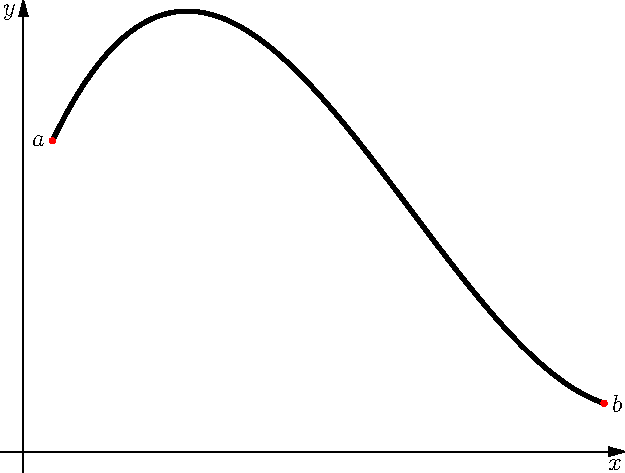
\includegraphics{./figures/1.1.pdf}
    
    \caption{Graph}
\end{figure}

\clearpage

This is not the graph of the function we're using the function we're actually using is $f(x) = \OurFunc$ for future convenice

%    \centering
%    %\includegraphics[width=0.5\textwidth]{fig1.png}
%    \caption{Example image}
%    \label{fig:image}
\chapter{Where Do We Start?}
Before we tackle getting the length of $\OurFunc$ we should start with a simpler function we already know how to get the length of.

\begin{figure}[h]
    \centering
    
    \includegraphics[width=\textwidth]{./figures/2.1.pdf}
    
    \caption{Graph of $y = \frac{4}{3}x$}
\end{figure}

Using the Pythagorean theorem you should've gotten that the length of the function from $a$ to  $b$ is $\sqrt{(b-a)^2 + (\frac{4}{3}b - \frac{4}{3}a)^2}$

In fact for any linear function $f(x) = kx$ the equation for length is

$$\ell = \sqrt{(b-a)^2 + (f(b) - f(a))^2}$$

\section{How is this useful?}
Well we could make an approximation based on distances of straight lines and we could make that approximation more and more accurate the smaller the horizontal length of the lines. Then to get the total length we would add the length af all the little lines.

\clearpage

\begin{figure}[h]
    \centering
    \begin{minipage}{0.45\textwidth} % Adjust width to fit your needs
        \centering
        \includegraphics[width=\textwidth]{./figures/2.2.pdf}
    \end{minipage}
    \hfill
    \begin{minipage}{0.45\textwidth} % Adjust width to fit your needs
        \centering
        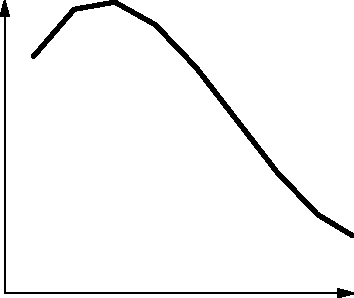
\includegraphics[width=\textwidth]{./figures/2.3.pdf}
    \end{minipage}
	\caption{Visual of function approximation}
\end{figure}


We can create a function that evaluates the sum of the lengths of all the lines ($\ell$) inside the interval of $a$ and $b$
$$S(a,b,\ell)$$

\section{First how do we evaluate $\ell$?}
Before we can evaluate $S$ we need to know $\ell$ at any point which will be defined as $\sqrt{dx^2 + dy^2}$ 
\subsection{How do we evaluate $dx$ and $dy$?}

\begin{figure}[h]
	\centering
	\begin{minipage}{0.45\textwidth} % Adjust width to fit your needs
		\centering
		\includegraphics[width=\textwidth]{./figures/2.4.1.pdf}
	\end{minipage}
	\hfill
	\begin{minipage}{0.45\textwidth} % Adjust width to fit your needs
		\centering
		\includegraphics[width=\textwidth]{./figures/2.4.pdf}
	\end{minipage}
	\caption{Visual of $dx$ and $dy$ getting smaller}
\end{figure}
We can think of $dx$ as a tiny change in $x$ at a certain $x$ but for now is basically just the step size and $dy$ as the change in $y$ at $x$

Botk the approximation of the equation and $S$ get more accurate as $dx$ shrinks closer to $0$. The mathematical term for a variable approaching a certain value is a limit and the notation is as follows:
\[
	\lim_{x \to 0}
\]


Anything written on the right hand side is evaluated close to that value for example
\[
\lim_{x \to 3} \frac{(x-3)(x-2)}{(x-3)} = 1
\]
The is $1$ despite the fact that if you actually plug in 3 you divide by zero

Now that we have the notaion we can say that
\[
\lim_{dx \to 0} {f(x+dx)-f(x)} = dy
\]
So now we have a way to describe $dy$ in terms of $dx$. Let's get some examples
\begin{enumerate}
	\item 
		$$f(x) = \frac{4}{3}x$$
		\[
		\lim_{dx \to 0} {\frac{4}{3}(x+dx)-\frac{4}{3}(x)} = dy
		\]
		$$\frac{4}{3}x + \frac{4}{3}dx - \frac{4}{3}x$$
		$$dy = \frac{4}{3}dx$$
		What this equation is basically saying is that for every change in $x$ the Change in $y$ is that change multiplied by $\frac{4}{3}$
	\item
		$$f(x) = x^2$$
		\[
		\lim_{dx \to 0} {(x+dx)^2-x^2} = dy
		\]
		\[
		\lim_{dx \to 0} {x^2+2xdx+dx^2-x^2} = dy
		\]
		We can ignore the $dx^2$ since it goes to 0 very fast this will make more sense in the future when we divide by $dx$. In general we can ignore any $o(h)$ if \( \displaystyle \lim_{h \to 0} \frac{o(h)}{h} = 0\) in the future so
		$$dy = 2xdx$$
\end{enumerate}

Let's ensure that these make sense we already know that the length of the line $\frac{4}{3}x$ is $\sqrt{(b-a)^2 + (\frac{4}{3}b - \frac{4}{3}a)^2}$ across $a$ and $b$. 

If all the lengths are $\sqrt{dx^2 + dy^2} = \sqrt{dx^2 + (\frac{4}{3}dx)^2}$ and $dx$ is a change in $x$ we could say that the sum of all those changes over $a$ and $b$ is $b-a$.
Substitution would make it $\sqrt{(b-a)^2 + (\frac{4}{3}b - \frac{4}{3}a)^2}$ which is the same so it makes sense.

If we were to lower the step size it would make no differce since you'd be adding $dx = \frac{(b-a)}{2}$ twice giving us the same result.
%\begin{figure}[h]
%    \centering
%    
%    
%    
%    \caption{Visualization of the sums of the $dx$'s'}
%\end{figure}

Also as a generalization we'll say $dy = f'(x)dx$ which also means $\frac{dy}{dx}=f'(x)$ and $\frac{d}{dx}f(x)=f'(x)$ in this context $d$ is an operator that means a tiny change. We will call all of these the derivative which can be defined as:
\[
f'(x) = \lim_{h \to 0} \frac{f(x + h) - f(x)}{h}
\]
We can show why the $dx^2$ doesn't matter in the derivative of $x^2$
\[
	f'(x) = \lim_{h \to 0} \frac{(x+h)^2 - x^2}{h}
\]
\[
	f'(x) = \lim_{h \to 0} \frac{x^2 + 2xh + h^2 - x^2}{h}
\]
Canceling yields
\[
	f'(x) = \lim_{h \to 0} 2x + h
\]
And since $h$ approaches zero $f'(x) = 2x$

\chapter{Calculating $S$}
Our notation for $S$ is too clunky so lets clean it up by moving some symbols around. Let's also give it a name: Integration
$$\int_{a}^{b} \ell$$
But more important than that our definition doesn't provide any methods to calculate it. Let's start with some basic intuition.

If we are adding all instances of something within a boundary then Integrating $dx$ should give us the length of the boundary giving us.
$$\int_{a}^{b} dx = b-a$$

We can also reasonably assume that if we are integrating $dx$ times a coefficent $k$ then we should get the distance times that coefficent.
$$\int_{a}^{b} kdx = kb-ka$$
$$k\int_{a}^{b} dx = kb-ka$$

So what would happen is we tried $\int_{a}^{b} k$? We would get $k\infty$ since we are adding $k$ for all values between $a$ and $b$ which is infinite. So $dx$ is keeping the result finite by being a tiny difference which will add up to the whole change in $x$.

But what do we do about non-constant coefficents?

$$\int_{a}^{b} g(x)dx = ?$$

We could say that $g(x)=\frac{dy}{dx}$ giving us:

$$\int_{a}^{b} \frac{dy}{dx}dx = ?$$
If $\frac{dy}{dx} = f'(x)$ then $y = f(x)$.
The $dx$'s cancel giving us:

$$\int_{a'}^{b'} dy$$

Which is the total change in $y$ across the change in $x$. Note that the bounds are different because the start and end points are different with $y$ than with $x$. $a'$ and $b'$ are $f(a)$ and $f(b)$

\begin{figure}[h]
    \centering
    
	\includegraphics{./figures/3.1.pdf}
    
    \caption{Visualization of the total change in $y$}
\end{figure}

After some manipulation you reach the
\begin{center}
	\textbf{Fundemental Theorem of Calculus:}
\end{center}


\begin{center}
	\boxed{\int_{a}^{b} f'(x)dx = f(b)-f(a)}
\end{center}

\section{We need to go backwards}
We know how to fo from $f(x)$ to $f'(x)$ and as we'll find out it's relatively easy but not the other way around. As always let's start by doing something we already know the answer to.

$$\int_{a}^{b} 2xdx = b^2-a^2$$
we know $\frac{d}{dx}x^2 = 2x$ from the last chapter so the answer to the integral:
$$\int_{1}^{3} 2xdx = 3^2-1^2 = 8$$

Let't introduce some new notation the operator that lets us go from $f'(x)$ to $f(x)$ will be called the anti-derivative or the indefinite integral and it looks like the integral but without the bounds:
\[
\int f(x) \, dx
\]
$f(x)$ is what we're trying to go backwards from and $dx$ is the variable we're integrating with respect to. And in order to account for the dropped constant during differentiation we add a $+C$ so:
\[
\int f'(x) \, dx = f(x) + C
\]

\chapter{To go backwards we must go forward}
If we want to find out how to from a derivative to a normal function we're going to need to figure out how to get derivatives and go backwards from there. Also to solve our problem we're going to need to find the derivative of $\OurFunc$ to get our $dy$
\section{Rules of differentiation}
 In algebra we have three major operators addition, multiplication, and exponatiation we also have composition. In order to get the derivative and anti-derivative of $\OurFunc$ we must learn how all four work.
\subsection{Addition}
You can trivially convince yourself that the rule for addition is
\begin{center}
\boxed{\frac{d}{dx}f(x)+g(x) = f'(x) + g'(x)}
\end{center}

When adding both functions directly contribute to to $dy$
%\begin{figure}[h]
%    \centering
%    
%    
%    
%    \caption{Visualization of graph addition and change of $dy$}
%\end{figure}
%
$$dy=df+dg$$

\subsection{Multiplication}
The rule for multiplication is called the product rule and its:
\begin{center}
\boxed{\frac{d}{dx}f(x)g(x) = f'(x)g(x) + g'(x)f(x)}
\end{center}

Multiplication is a little more complicated and a geometric visual is easier to understand.


\begin{figure}[h]
    \centering
		\includegraphics{./figures/4.1.pdf}
    \caption{Visualization of geometric intuition for the product rule}
\end{figure}
The yellow areas are our change and the red is too small to matter.
A little confirmation if we follow the the product rule for $x^2$ we should get $2x$

$$\frac{d}{dx}x^2$$
$$\frac{d}{dx}xx$$
$$1x + 1x = 2x$$

\subsection{Composition}
The rule for composition is called the chain rule and its:
\begin{center}
\boxed{\frac{d}{dx}f(g(x)) = g'(x)f'(g(x))}
\end{center}

A symbolic proof we want to find $df$ in terms of $dx$
$$f(g(x))$$
$$\frac{df}{dx} = \frac{df}{dg}\frac{dg}{dx}$$
$dg$'s cancel

A more intuative look at why whis is the case is that we set $df$ in terms of $g(x)$ and $dg$ then Substitute out all $g(x)$'s and $dg$'s to get the derivative in terms of $x$ and $dx$. Let's look at a problem:
a factory can produces copper wire for every kg of copper it has it can produce that amount squared. The factory buys its copper at 2kg for 1$m$ $m$ is dollar. How much wire do you get per dollar?
\subsubsection{Step 1}
Set up equations
$$dw = 2cdc$$
$$dc = 2dm$$
$$c = 2m$$

\subsubsection{Step 2}
	Substitution
	$$dw = 2(2m)2dm$$
	$$dw = 8mdm$$
	$$\frac{dw}{dm} = 8m$$
	At any given doller amount the amount of meters of copper wire per dollar is 8 times the dollar you're on. I encourage you to construct a similar problem to further confirm why this method works.

\subsection{Recap}
\itemize
	\item Addition:
	$$\frac{d}{dx}f(x)+g(x) = f'(x) + g'(x)$$
	\item Multiplication:
	$$\frac{d}{dx}f(x)g(x) = f'(x)g(x) + g'(x)f(x)$$
	\item Composition:
	$$\frac{d}{dx}f(g(x)) = g'(x)f'(g(x))$$

\chapter{Yes exponents need their own chapter}
The final differentiation rule we need is an exponent rule:
$$\frac{d}{dx}f(x)^{g(x)} = ?$$
First let's make some notaion more compound $\frac{dy}{dx}$ will now be $y'$. 
\section{The product rule and Implicit Differentiation}
We'll also need to figure out some new techniques which is having $y$ on both sides of the equation this is part of wider technique called Implicit differentiation. To sanity check this technique we'll double check if we can get the product rule.

$$y=f(x)g(x)$$
$$y'=f(x)'g(x)+f(x)g'(x)$$
$$y'=\left(\frac{f'(x)}{f(x)} + \frac{g'(x)}{g(x)}\right)(f(x)g(x))$$
$$y'=\left(\frac{f'(x)}{f(x)} + \frac{g'(x)}{g(x)}\right)y$$
$$\frac{y'}{y}=\frac{f'(x)}{f(x)} + \frac{g'(x)}{g(x)}$$

Notice how in order to achive the final form we need to apply an operation on both sides that has the following properties:
\begin{enumerate}
	\item It's derivative looks like $\frac{y'}{y}$ or $\frac{1}{x}$
	\item It seperates products into its factors such that $f(ab) = f(a) + f(b)$
\end{enumerate}

We don't yet know of a function or operation that satifies the first condition but we do know that logarithms satisfy the second condition. So we can rewrite as:
$$\log(y)=\log(f(x)g(x))$$
$$\log(y)=\log(f(x))+ \log(g(x))$$
\subsection{Derivative of a logarithm}
Now we ln need to find the derivative of logarithms and maybe we could manipulate them to give us the derivative $\frac{y'}{y}$ while still perserving the seperation of products property.

\[
\lim_{h \to 0} \frac{\log_k(x+h)-\log_k(x)}{h} = ?
\]

This seems rather difficult it may be easier to set logarithms in the form of $k^y = x$ and then set the derivative in terms of $x$

\[
\lim_{h \to 0} \frac{k^{x+h}-k^x}{h}
\]

\[
\lim_{h \to 0} \frac{k^hk^{x}-k^x}{h}
\]

\[
\lim_{h \to 0} \frac{(k^h-1)k^{x}}{h}
\]

\[
\ k^x \lim_{h \to 0} \frac{k^h-1}{h}
\]

This is beyond the scope of the book but there is a value for $k$ such that \( \displaystyle \lim_{h \to 0} \frac{k^h-1}{h} = 1\).
We call this value $e$ and the we call $\log_e$ the natural logarithm $\ln$. A very nice property of the $e^x$ is that its derivative is also $e^x$. So let's solve the derivative of $\ln$

$$y = \ln(x)$$
$$e^y = x$$
$$e^ydy = dx$$
$$e^y\frac{dy}{dx} = 1$$
$$\frac{dy}{dx} = \frac{1}{e^y}$$
$$e^y = x$$
$$\frac{dy}{dx} = \frac{1}{x}$$
$$\frac{d}{dx}\ln(x) = \frac{1}{x}$$

Coincidentally this satisfies both properties required to get the product rule through implicit differentiation. Let's go through it then:

$$y=f(x)g(x)$$
$$\ln(y)=\ln(f(x)g(x))$$
$$\ln(y)=\ln(f(x))+\ln(g(x))$$
$$\frac{y'}{y}=\frac{f'(x)}{f(x)} + \frac{g'(x)}{g(x)}$$
$$y'=\left(\frac{f'(x)}{f(x)} + \frac{g'(x)}{g(x)}\right)y$$
$$y=f(x)g(x)$$
$$y'=\left(\frac{f'(x)}{f(x)} + \frac{g'(x)}{g(x)}\right)(f(x)g(x))$$
$$y'=f(x)'g(x)+f(x)g'(x)$$

We can reasonably say that our implicit differentiation works.

\section{Finding the exponent rule}
We could start by changing the the expression to one of products and sums using the natural logarithm

$$y=f(x)^{g(x)}$$
$$\ln(y)=\ln\left(f(x)^{g(x)}\right)$$
$$\ln(y)=g(x)\ln(f(x))$$
$$\frac{y'}{y}=g(x)'\ln(f(x)) + g(x)\frac{f'(x)}{f(x)}$$
$$y'=\left(g(x)'\ln(f(x)) + g(x)\frac{f'(x)}{f(x)}\right)y$$
$$y=f(x)^{g(x)}$$
$$y'=\left(g(x)'\ln(f(x)) + g(x)\frac{f'(x)}{f(x)}\right)f(x)^{g(x)}$$
$$y'=g(x)'\ln(f(x))f(x)^{g(x)} + g(x)f'(x)f(x)^{g(x)-1}$$

So our exponent rule is this monster (most calculus classes won't expect you to know this rule):
\begin{center}
\boxed{\frac{d}{dx}f(x)^{g(x)} =g(x)'\ln(f(x))f(x)^{g(x)} + g(x)f'(x)f(x)^{g(x)-1}}
\end{center}

Let's double check  by putting $e^x$ and $x^2$ through the rule which should return $e^x$ and $2x$ respectively.

Checking $e^x$:
$$f(x) = e$$
$$g(x) = x$$
$$1\ln(e)e^x + x \cdot 0e^{x-1}$$
$$1\ln(e)e^x = e^x$$

Checking $x^2$:
$$f(x) = x$$
$$g(x) = 2$$
$$0\ln(x)x^2 + 2 \cdot 1x^{2-1}$$
$$2x^1 = 2x$$
In fact if $f(x) = x$ and $g(x)$ is any real number $r$ we can derive
\begin{center}
	\textbf{The Power Rule:}
\end{center}

\begin{center}
	\boxed{\frac{d}{dx}x^r = rx^{r-1}}
\end{center}

\chapter{Now we can solve our initial problem}

In case you forgot our initial problem was to find the arc length of $\OurFunc$ from $a$ to $b$. We figured out in previuos chapters we write this problem as:

$$\int_{a}^{b} \sqrt{dx^2 + dy^2}$$

We can simplify $\sqrt{dx^2 + dy^2}$ by setting $dy$ in terms of $dx$ then extractiong $dx$ outside of the square root

$$ dy = f'(x)dx $$
$$\sqrt{dx^2 + (f'(x)dx)^2}$$
$$\sqrt{dx^2 + f'(x)^2dx^2}$$
$$\sqrt{dx^2 (1 + f'(x)^2)}$$
$$\sqrt{1 + f'(x)^2}dx $$

Now we need to find $f'(x)$ from $f(x) = \OurFunc$ we can use our power rule for this and product rule for this.
$$r = \frac{3}{2}$$
$$\frac{d}{dx} x ^{\frac{3}{2}} = \frac{3}{2}x^{\frac{1}{2}}$$
Using the product rule
$$f(x) = x ^{\frac{3}{2}}$$
$$g(x) = \frac{4}{3}$$
$$\frac{d}{dx}\OurFunc = \frac{4}{3} \cdot \frac{3}{2}x ^{\frac{1}{2}} + 0x^\frac{3}{2}$$
$$\frac{d}{dx}\OurFunc = 2x^\frac{1}{2}$$

If we plug these in to our integral we get:
$$\int_{a}^{b} \sqrt{1 + (2\sqrt{x})^2}dx$$
$$\int_{a}^{b} \sqrt{1 + 4x}dx$$
Now we need to modify $\sqrt{1 + 4x}dx$ into something that's easier to integrate. To do this we can use a sort of backwards chainrule. We'll define a $u = 1+4x$ and get $dx$ in terms of $u$ and intgrate
$$u = 1+4x$$
$$du = 4dx$$
$$dx = \frac{du}{4}$$

$$\int \sqrt{1+4x}dx$$
$$\int \frac{\sqrt{u}}{4}du$$
$$\int \frac{1}{4}u^{\frac{1}{2}}du$$
%$$\frac{1}{4}\int u^{\frac{1}{2}}du$$

We can generate power rule for integration by doing the previous power rule's steps backwards
$$\int x^rdx = \frac{x^{r+1}}{r+1} + C$$
$$\int \frac{1}{4}u^{\frac{1}{2}}du = \frac{1}{6}u^{\frac{3}{2}} + C$$
Finally we can solve our initial problem
$$\int_ {a'}^{b'} \frac{1}{4}u^{\frac{1}{2}}du$$
our new bounds are $a' = 1+4a$ and $b' = 1+4b$ so after substitution our full answer after is:
$$\int_{a}^{b} \sqrt{1 + 4x}dx = [\frac{1}{6}(1+4b)^{\frac{3}{2}}-\frac{1}{6}(1+4b)^{\frac{3}{2}}]$$
This is the equation for finding the arc length of the function $\OurFunc$ from $x=a$ to $x=b$
\chapter{Final Remarks}
The following are the concepts at the heart of calculus:
\begin{enumerate}
	\item The most powerful use of calculus is its ability to turn non-linear problems into many solvable linear problems as you've previously seen.
	\item The $d$ operator means a tiny change in whatever it is operating on $\frac{d}{dx}$ tells you that change in respect to $x$ which is why you are dividing by $dx$
	\item The definite integral $\int_{a}^{b}$ is a sum of all the things within the boundary $a$ and $b$ those things are definied by whatever comes after the integral. 
		It should be no suprise that the sum of all the differences within a boundary is the whole of the thing in the boundary hence why $\int_{a}^{b} dx = b - a$.

	\item Do not think of the definite integral and anti-derivative as the same thing one is the sum over an interval the other is an operation that coverts $f'(x)$ to $f(x)$. Their relationship is that the anti-derivative makes computing the definite intergral possible.
	\item A more broad interpretation of fundemental theorem of calculus $\int_{a}^{b} f'(x)dx = f(b)-f(a)$ is that the sum of everything within a domain ($\omega$) is equal to the sum of the anti-derivative along the boundary of the domain ($\partial \omega$).

You will encounter this concept expressed in different ways in other theorems such as Stoke's Theorem or Green's Theorem but they all basically say the same thing.
\item A limit is basically just getting infinitely close to a value from all directions and sometimes a specific direction is specified.
\end{enumerate}

Finally I want you to consider the information derivatives and anti-derivatives give us about a function and how we can use that information to solve problems like generating a distance traveled function $d(t)$ given the function $v(t)$ which gives the velocity at time $t$.



\end{document}

